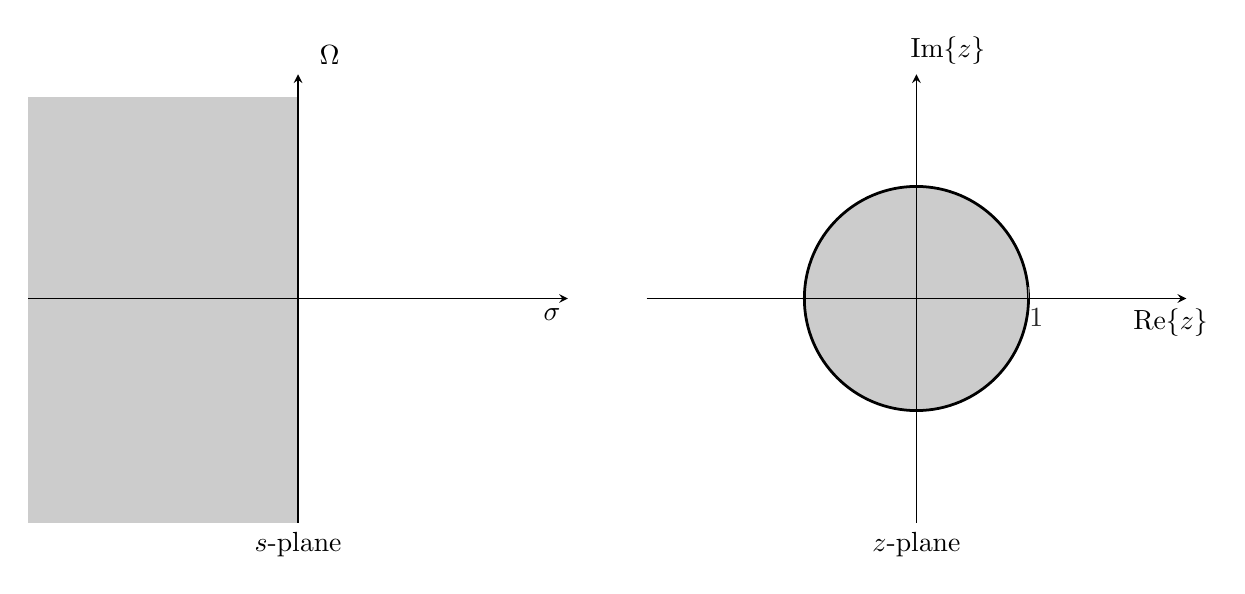
\begin{tikzpicture}
\begin{axis}[
name=plot1,
axis equal,
axis lines*=middle,
enlargelimits = false, clip=true,
axis on top=true,
axis line style={->,>=stealth},
xlabel={$\sigma$},
ylabel={$\Omega$},
every axis x label/.style={
	at={(ticklabel* cs:1)},
	xshift=-0.2cm,
	anchor=north,
},
every axis y label/.style={
	at={(ticklabel* cs:1)},
	xshift=0.4cm,
	%yshift=0.35cm,
	anchor=south,
},
every outer x axis line/.append style={white!15!black},
every x tick label/.append style={font=\color{white!15!black}},
xmin=-2, xmax=2,
ymin=-2, ymax=2,
xtick=\empty,
ytick=\empty,
every outer y axis line/.append style={white!15!black},
every y tick label/.append style={font=\color{white!15!black}},
legend style={draw=white!15!black,fill=white,legend cell align=left}]

\fill[black!20] (axis cs:-3, -2) rectangle (0, 1.8);

\end{axis}

\begin{axis}[
name=plot2,
axis equal,
at=(plot1.east), anchor=west, xshift=1cm,
axis lines*=middle,
enlargelimits = false, clip=true,
axis on top=true,
axis line style={->,>=stealth},
xlabel={$\mathrm{Re}\{z\}$},
ylabel={$\mathrm{Im}\{z\}$},
every axis x label/.style={
	at={(ticklabel* cs:1)},
	xshift=-0.2cm,
	anchor=north,
},
every axis y label/.style={
	at={(ticklabel* cs:1)},
	xshift=0.4cm,
	%yshift=0.35cm,
	anchor=south,
},
every outer x axis line/.append style={white!15!black},
every x tick label/.append style={font=\color{white!15!black}},
xmin=-2, xmax=2,
ymin=-2, ymax=2,
xtick=1,
ytick=\empty,
xticklabel style={xshift=0.1cm},
every outer y axis line/.append style={white!15!black},
every y tick label/.append style={font=\color{white!15!black}},
legend style={draw=white!15!black,fill=white,legend cell align=left}]

\draw[black, fill=black!20, line width=1pt] (axis cs:0,0) circle [radius=1];

\end{axis}

\node[below] at (plot1.south) {$s$-plane};
\node[below] at (plot2.south) {$z$-plane};
\end{tikzpicture}